% !TeX root = main.tex
% Completed draft001 final-evaluation aggregates; no event/model replay.
\subsection{Observed final-evaluation spectra}

The final-evaluation sample contains 9,049 signal and 698 background physical
event groups. The frozen validation-background thresholds are 0.746724 for ABCD
and 0.860891 for BCD at seed 42 (rounded for display). The high category uses
scores at or above the respective full-precision threshold. Both spectra use
signed yield weights divided by the 0.2 evaluation assignment probability.

The common baseline has expected signal/background yields of 2.771/2.355 at
10~fb$^{-1}$. ABCD retains 96.8\% of the signal and 51.1\% of the background;
BCD retains 94.6\% and 46.8\%, respectively. At these separately frozen cuts,
BCD rejects more of each process. These are signed-yield retentions, not the
absolute-weight acceptances used to define the validation cuts. They need not
equal the nominal 50\% validation-background acceptance.

\begin{table*}[tbp]
\caption{Signed-yield diagnostic at seed 42. Errors are grouped MC standard
errors at fixed networks and cuts. Retention errors include the shared-event
before/after covariance. Counts below are physical expectations, not MC occupancy.}
\label{tab:yields}
\centering
\begin{tabular}{llrr}
\toprule
Process & Selection & Signed yield & Retention (\%) \\
\midrule
Signal & Before & $2.7710\pm0.0293$ & --- \\
 & ABCD high & $2.6824\pm0.0288$ & $96.80\pm0.19$ \\
 & BCD high & $2.6215\pm0.0285$ & $94.60\pm0.24$ \\
Background & Before & $2.3553\pm0.1683$ & --- \\
 & ABCD high & $1.2027\pm0.1202$ & $51.06\pm3.57$ \\
 & BCD high & $1.1012\pm0.1156$ & $46.75\pm3.57$ \\
\bottomrule
\end{tabular}
\end{table*}

Figure~\ref{fig:draft001-yields} shows the simulated signal concentrated near
125~GeV. The interval $[120,130)$~GeV contains 87.9\% of its baseline signed yield,
compared with 88.6\% after the ABCD cut and 88.5\% after the BCD cut. Both selections
retain the main signal region. These coarse bins do not establish a shift in peak
position, a change in detector resolution or a change in the physical Higgs width.

\begin{figure*}[tbp]
\centering
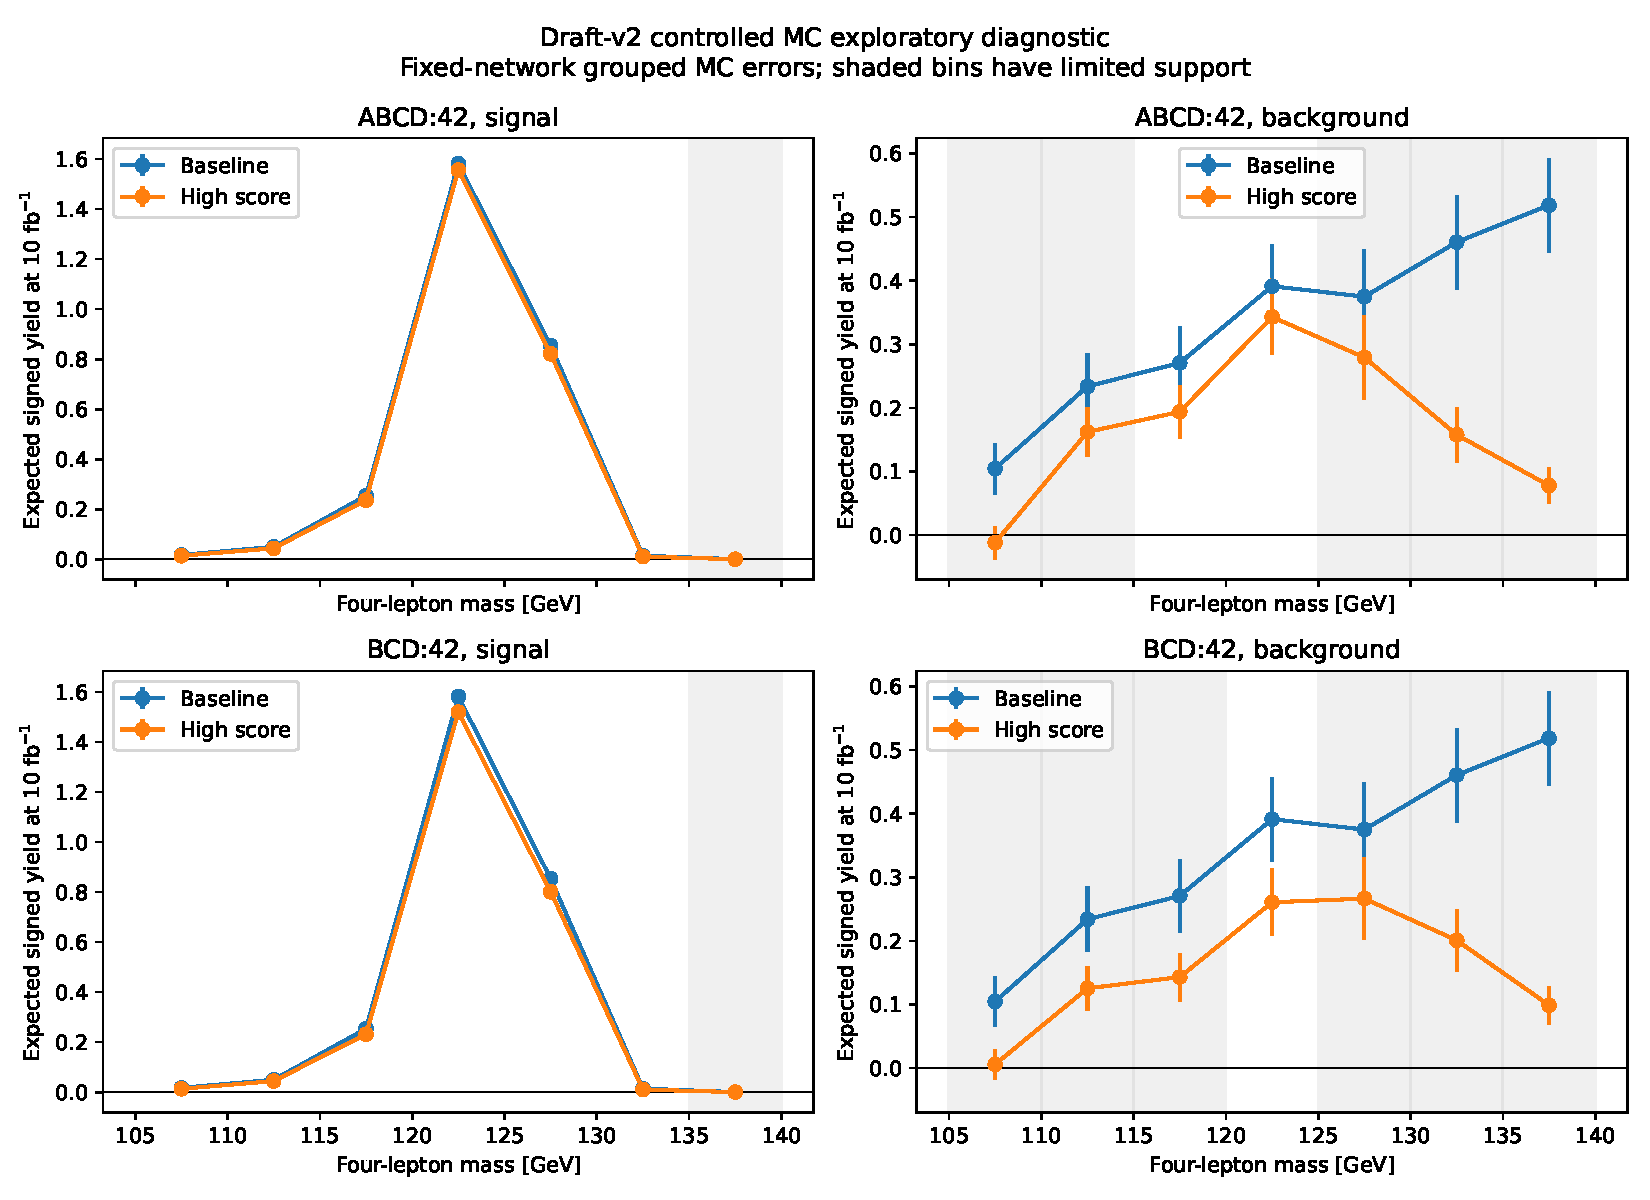
\includegraphics[width=0.88\textwidth]{figures/draft001/mass-yields.pdf}
\caption{Draft001 final-evaluation signed mass spectra at 10~fb$^{-1}$ before and
after the frozen high-score cuts. ABCD is above and BCD below, both at seed 42;
signal is left and background right. Error bars use grouped MC variance.
Shading flags low-support bins; negative yields remain visible. These seven
half-open 5~GeV display bins do not enter the likelihood, which uses one mass
interval and both score categories. Before and after curves share events.}
\label{fig:draft001-yields}
\end{figure*}

The baseline background is broad and nonuniform over the selected window. Its
signed fraction in $[120,130)$~GeV increases from 32.5\% before the cut to 51.8\%
for ABCD and 47.9\% for BCD. Its $[135,140)$~GeV fraction decreases from 22.0\% to
6.5\% and 9.0\%, respectively. Thus the selection changes background shape as well
as total yield. This is evidence of mass dependence of the frozen selections
on this MC population despite the omission of explicit mass input. It does not
identify a unique responsible feature or establish a physical background resonance.

\begin{figure*}[tbp]
\centering
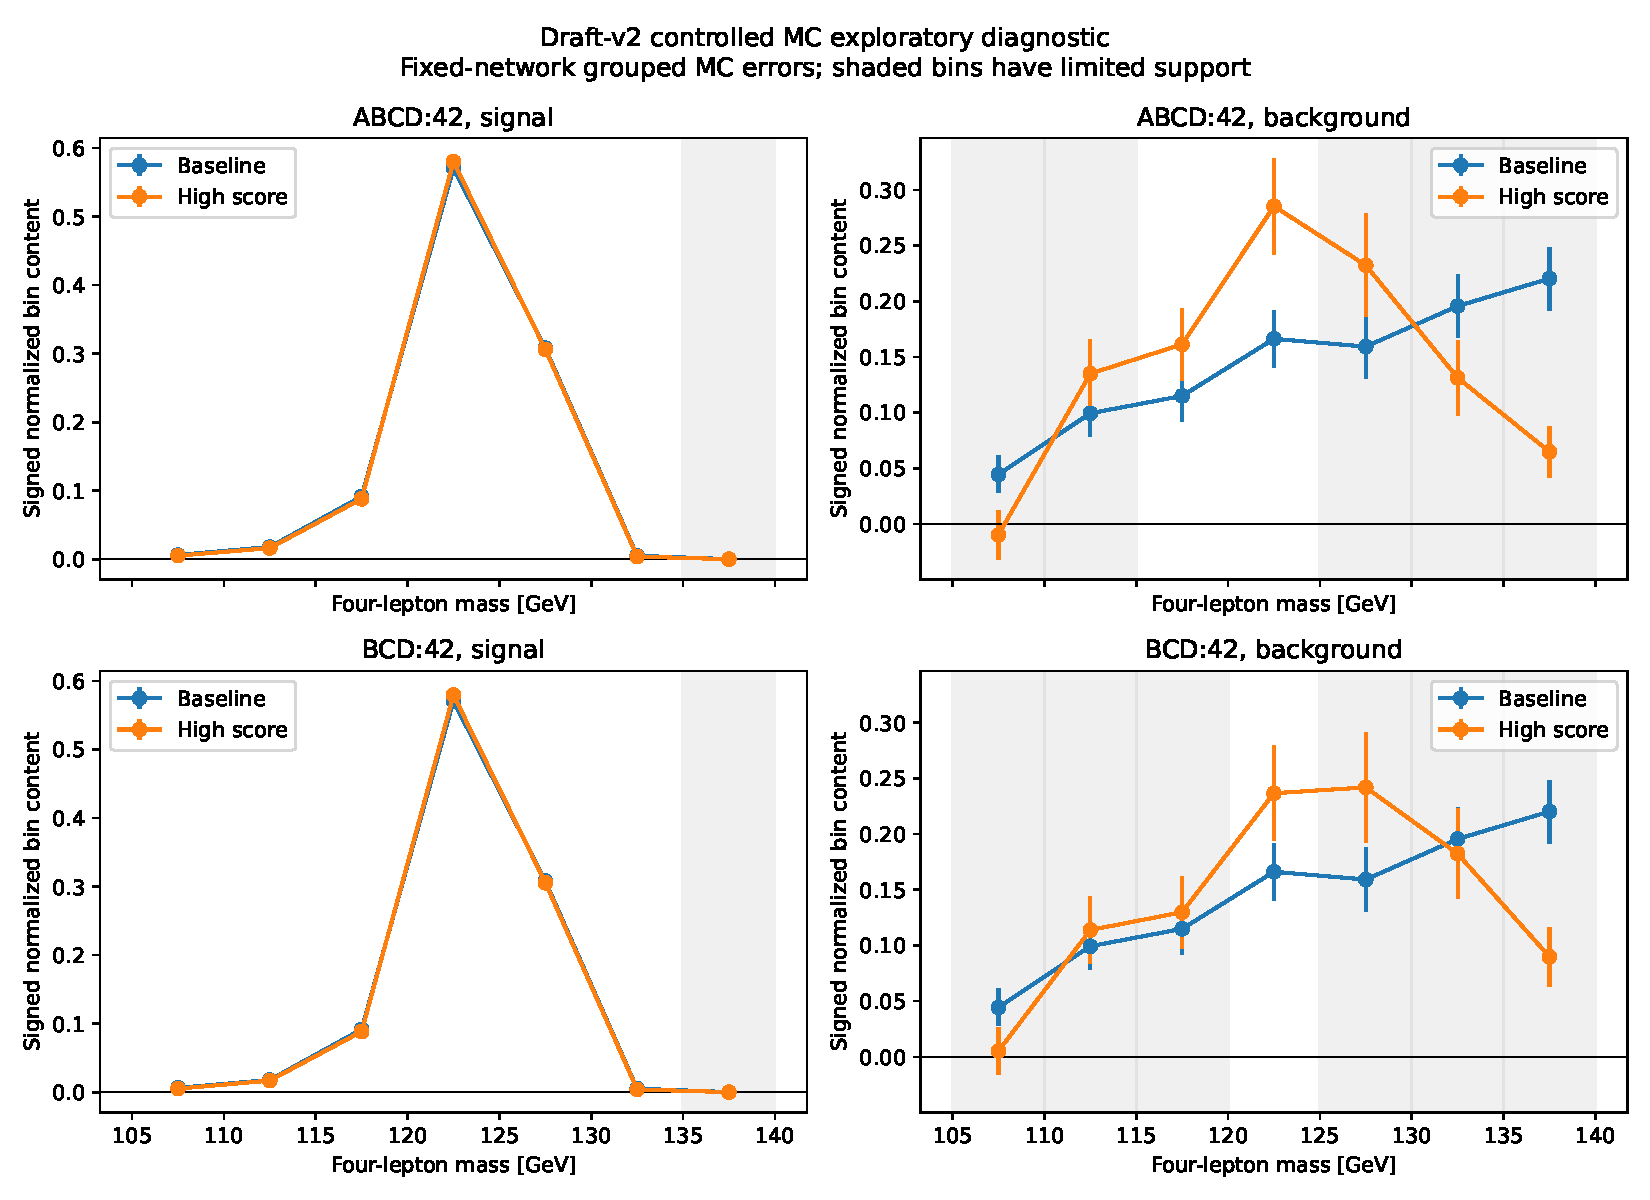
\includegraphics[width=0.88\textwidth]{figures/draft001/mass-shapes.pdf}
\caption{Draft001 before/after shapes for the same final-evaluation population
and models as Figure~\ref{fig:draft001-yields}. Each process and selection is
normalized by its own positive signed total. Errors propagate the shared
normalization; the report retains the full joint before/after shape covariance.
The error bars are therefore not independent measurements to subtract in a
shape comparison. Low-support and negative bins are retained without smoothing,
clipping or rebinning. A signed shape is not necessarily a probability density.}
\label{fig:draft001-shapes}
\end{figure*}

In particular, the selected ABCD background bin $[105,110)$~GeV has a negative
signed yield, and several background display bins have limited effective support.
The signal tail $[135,140)$~GeV also has very low occupancy. These local warnings
remain visible even though the wider mass-integrated categories satisfy the T1
support requirements. Neither the small tail differences nor the stronger visible
signal enrichment establish calibrated inference gains. All spectral errors
condition on the frozen networks and cuts; they omit threshold estimation,
independent retraining and coverage uncertainty.
